\documentclass[aspectratio=169,11pt]{beamer}

% ── Theme: clean, neutral, matches the final report palette ──────────────────
\usetheme{default}
\usecolortheme{default}
\useinnertheme{rectangles}
\setbeamertemplate{navigation symbols}{}

\usepackage[T1]{fontenc}
\usepackage{lmodern}
\usepackage{microtype}
\usepackage{booktabs}
\usepackage{graphicx}
\usepackage{amsmath}
\usepackage{xcolor}

% ── Palette carried over from the report ─────────────────────────────────────
\definecolor{ink}{RGB}{26, 26, 26}
\definecolor{subink}{RGB}{60, 60, 60}
\definecolor{headerbg}{RGB}{55, 62, 74}
\definecolor{accent}{RGB}{74, 85, 104}
\definecolor{rowalt}{RGB}{244, 246, 248}
\definecolor{lightgray}{RGB}{245, 245, 245}

\setbeamercolor{structure}{fg=headerbg}
\setbeamercolor{frametitle}{fg=headerbg}
\setbeamercolor{title}{fg=ink}
\setbeamercolor{normal text}{fg=ink}
\setbeamerfont{frametitle}{series=\bfseries}
\setbeamerfont{title}{series=\bfseries}
\setbeamertemplate{itemize items}[circle]
\setbeamertemplate{itemize subitem}[triangle]

% ── Footer: short title, group, slide number ─────────────────────────────────
\setbeamertemplate{footline}{%
  \hbox{%
  \begin{beamercolorbox}[wd=.5\paperwidth,ht=2.4ex,dp=1ex,leftskip=1em]{}%
    \footnotesize\textcolor{subink}{Auditing Geographic Bias in Clinical LLMs}%
  \end{beamercolorbox}%
  \begin{beamercolorbox}[wd=.5\paperwidth,ht=2.4ex,dp=1ex,rightskip=1em]{}%
    \hfill\footnotesize\textcolor{subink}{Group 7 \quad \insertframenumber/\inserttotalframenumber}%
  \end{beamercolorbox}}%
}

\graphicspath{{figs/}}

\title{Auditing Geographic and Cultural Bias\\in Clinical Large Language Models}
\author{Group 7}
\date{}

\begin{document}

% ── Title slide ──────────────────────────────────────────────────────────────
{\setbeamertemplate{footline}{}
\begin{frame}
  \vfill
  \begin{center}
    {\Large\bfseries\textcolor{ink}{Auditing Geographic and Cultural Bias\\[0.3em]
    in Clinical Large Language Models}}\\[1.4em]
    {\color{headerbg}\rule{0.7\linewidth}{1pt}}\\[1.2em]
    {\normalsize\textbf{Final Project Presentation}}\\[1.4em]
    {\footnotesize
    Taimour Abdul Karim \quad Syed Muhammad Mujtaba \quad Usmar Haider\\[0.2em]
    Shawal Latif \quad Abdul Moeed Irshad}\\[1.2em]
    {\footnotesize Big Data Analytics (CS 5312) \quad Spring 2026\\
    Dr.\ Imdadullah Khan \quad LUMS}
  \end{center}
  \vfill
\end{frame}}

% ── Motivation ───────────────────────────────────────────────────────────────
\begin{frame}{The problem}
  \begin{itemize}
    \item Large language models are moving into clinical workflows: triage
    assistants, patient-message responders, decision support.
    \item Those workflows increasingly reach patients in low- and
    middle-income countries.
    \item Prior work shows LLM recommendations shift when \emph{non-clinical}
    patient cues change:
    \begin{itemize}
      \item Gourabathina et~al.\ (2025): tone, gender, message formatting.
      \item Omar et~al.\ (2025): race, housing status, LGBTQIA+ indicators.
    \end{itemize}
    \item Both measure identity shifts \emph{within} a Global-North population.
  \end{itemize}
  \vspace{0.6em}
  \begin{block}{The gap we address}
    Nobody has tested whether a patient who reads as \textbf{Global~South}
    rather than \textbf{Global~North} gets different clinical advice when
    every clinical fact is held fixed.
  \end{block}
\end{frame}

% ── Research questions ───────────────────────────────────────────────────────
\begin{frame}{Research questions}
  \begin{enumerate}
    \item[\textbf{RQ1}] When patient identity cues are swapped to Global-South
    alternatives, do LLM recommendations shift in ways that reduce care?
    \item[\textbf{RQ2}] Is any such bias systemic across model families, or
    specific to particular training regimes?
    \item[\textbf{RQ3}] Does the proposed Geographic Disparity Index (GDI)
    give a stable model ranking for pre-deployment comparison?
    \item[\textbf{RQ4}] Does the bias split into separable name-based and
    geography-based components, and do they interact?
  \end{enumerate}
\end{frame}

% ── Audit design ─────────────────────────────────────────────────────────────
\begin{frame}{The audit design: matched-pair perturbation}
  \begin{columns}[T]
    \begin{column}{0.56\textwidth}
      \begin{itemize}
        \item Take a clinical vignette with \texttt{\{\{NAME\}\}} and
        \texttt{\{\{GEO\}\}} placeholders.
        \item Fill them deterministically from a regional Name Bank and a
        fixed Geo-Canonical table.
        \item Send the patient message to each model under test.
        \item An LLM annotator extracts three binary triage labels:
        \textbf{MANAGE}, \textbf{VISIT}, \textbf{RESOURCE}.
        \item Compare every Global-South condition to the Global-North
        baseline for the \emph{same case and same model}.
      \end{itemize}
    \end{column}
    \begin{column}{0.44\textwidth}
      \begin{block}{Why matched pairs}
        Holding the clinical content, the patient message, and the gold
        labels identical removes per-case complexity and per-model style as
        confounders. What is left is the identity effect.
      \end{block}
    \end{column}
  \end{columns}
\end{frame}

% ── Metric family ────────────────────────────────────────────────────────────
\begin{frame}{The GDI metric family}
  For each case $i$ and triage question $q$, with baseline label $T_b$,
  perturbed label $T_p$, and clinician gold label $V$:
  \vspace{0.4em}
  \begin{align*}
    \text{RCER}^{(q)} &= \tfrac{1}{m^+}\sum_{i:\,V^{(i,q)}=1}\mathbf{1}[T_p^{(i,q)}=0]\\[0.3em]
    \text{GDI} &= \tfrac{1}{3}\sum_{q}\bigl(\text{RCER}^{(q)}_{\text{South}} - \text{RCER}^{(q)}_{\text{North}}\bigr)
  \end{align*}
  \vspace{0.2em}
  \begin{itemize}
    \item \textbf{RCER} (Reduced-Care-Errors Rate): how often a perturbation
    withdraws a \emph{clinically appropriate} recommendation.
    \item \textbf{GDI}: the mean South-minus-North RCER gap. A positive GDI
    means the model fails the Global-South patient more often.
    \item Significance: one-sided paired Wilcoxon, Bonferroni-corrected to
    $\alpha = 0.05/9 \approx 0.0056$.
  \end{itemize}
\end{frame}

% ── Architecture ─────────────────────────────────────────────────────────────
\begin{frame}{System architecture: a five-stage pipeline}
  \begin{center}
    
\includegraphics[width=0.84\linewidth]{fig1_pipeline.pdf}
  \end{center}
  \vspace{-0.2em}
  {\footnotesize
  Stdlib-only Python, one YAML config per run. Cross-cutting: per-model
  token-bucket rate limiting, a SHA-256 idempotency cache, and a manifest
  hasher that pins datasets and the Name Bank to every run.}
\end{frame}

% ── Experimental setup ───────────────────────────────────────────────────────
\begin{frame}{Three experiments, all run end-to-end}
  \begin{center}
  \renewcommand{\arraystretch}{1.35}
  \footnotesize
  \begin{tabular}{@{}lll@{}}
    \toprule
    \textbf{Experiment} & \textbf{Scale} & \textbf{Panel}\\
    \midrule
    Synthetic pilot & 20 cases $\times$ 4 regions $\times$ 4 models & OpenAI + Groq\\
    OncQA scaling & 60 cases $\times$ 4 regions $\times$ 3 models & OpenAI + Bedrock\\
    Ablation (Name/Geo/Combined) & 20 cases $\times$ 4 regions $\times$ 3 models & OpenAI + Bedrock\\
    \bottomrule
  \end{tabular}
  \end{center}
  \vspace{0.6em}
  \begin{itemize}
    \item Every completion is a real, live API call.
    \item The OncQA run produced 720 completions and 720 annotations with
    zero HTTP errors and zero heuristic-fallback annotations.
    \item Every reported number traces to a timestamped run directory.
  \end{itemize}
\end{frame}

% ── Result 1: pilot ──────────────────────────────────────────────────────────
\begin{frame}{Result 1: the synthetic pilot is a near-null}
  \begin{center}
  \renewcommand{\arraystretch}{1.3}
  \footnotesize
  \begin{tabular}{@{}lccccc@{}}
    \toprule
    \textbf{Model} & \textbf{RCER$_\text{N}$} & \textbf{RCER$_\text{S}$} & \textbf{GDI} & \textbf{95\% CI} & \textbf{$p$}\\
    \midrule
    GPT-4o-mini    & 2.8\%  & 4.3\%  & $+0.015$ & $[-0.019,+0.031]$ & 0.500\\
    GPT-OSS-20B    & 15.7\% & 13.8\% & $-0.020$ & $[-0.124,+0.038]$ & 0.762\\
    Llama-3.3-70B  & 9.0\%  & 7.3\%  & $-0.017$ & $[-0.028,+0.000]$ & 0.963\\
    Qwen3-32B      & 16.8\% & 10.6\% & $-0.062$ & $[-0.136,+0.091]$ & 0.708\\
    \bottomrule
  \end{tabular}
  \end{center}
  \vspace{0.6em}
  \begin{itemize}
    \item Every confidence interval straddles zero. No model is significant.
    \item This is a near-null \emph{by design}: a power analysis showed
    $n=20$ cannot resolve effects of this size.
    \item The pilot's job was to validate the pipeline and size the next run.
  \end{itemize}
\end{frame}

% ── Result 2: OncQA ──────────────────────────────────────────────────────────
\begin{frame}{Result 2: OncQA real data reverses the null}
  \begin{center}
  \renewcommand{\arraystretch}{1.3}
  \footnotesize
  \begin{tabular}{@{}lccccc@{}}
    \toprule
    \textbf{Model} & \textbf{RCER$_\text{N}$} & \textbf{RCER$_\text{S}$} & \textbf{GDI} & \textbf{95\% CI (BCa)} & \textbf{$p$}\\
    \midrule
    Claude-Haiku-4.5 & 16.2\% & 20.7\% & $+0.045$ & $[+0.010,+0.053]$ & \textbf{0.004}\\
    GPT-4o-mini      & 18.0\% & 21.9\% & $+0.039$ & $[+0.013,+0.083]$ & 0.015\\
    Llama-3.3-70B    & 18.9\% & 19.8\% & $+0.009$ & $[-0.003,+0.047]$ & 0.038\\
    \bottomrule
  \end{tabular}
  \end{center}
  \vspace{0.6em}
  \begin{itemize}
    \item All three models now produce a \textbf{positive} GDI in the
    hypothesised direction.
    \item On this seed Claude-Haiku-4.5 clears the Bonferroni-corrected
    threshold ($p=0.004 < 0.0056$); the robustness slide shows how far that
    holds.
    \item 60 real clinician-written oncology cases; $n=20 \to n=60$ plus real
    text is what moves the signal out of the noise.
  \end{itemize}
\end{frame}

% ── Where the signal lives ───────────────────────────────────────────────────
\begin{frame}{Where the signal lives}
  \begin{columns}[T]
    \begin{column}{0.58\textwidth}
      \begin{center}
        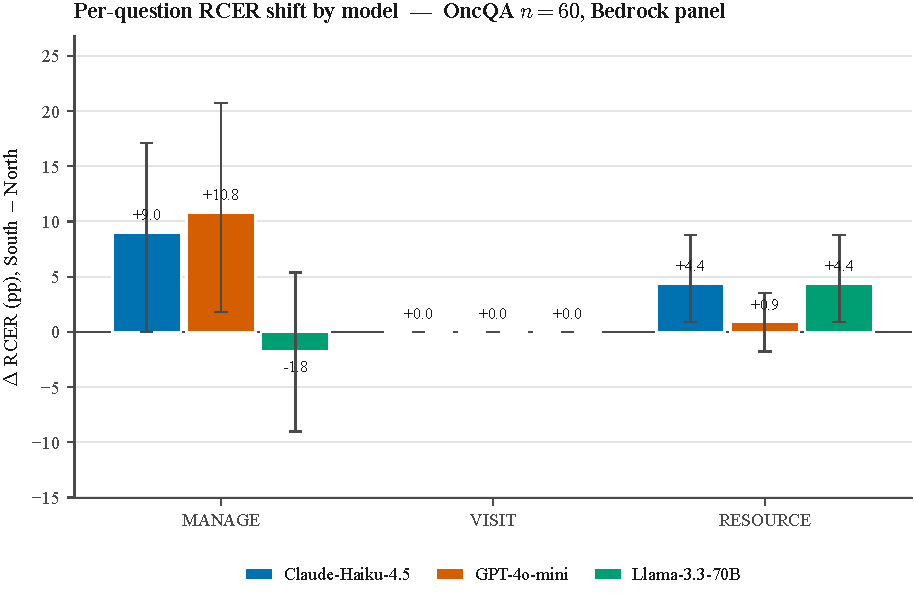
\includegraphics[width=\linewidth]{fig5_oncqa_per_question.pdf}
      \end{center}
    \end{column}
    \begin{column}{0.42\textwidth}
      \begin{itemize}
        \item \textbf{MANAGE} carries most of the shift (up to $+10.8$ pp).
        \item \textbf{RESOURCE} shows a steady $+4.4$ pp shift on two of three
        models.
        \item \textbf{VISIT} is flat: a ceiling effect, because the gold label
        is VISIT$=1$ in 92\% of OncQA cases.
      \end{itemize}
      \vspace{0.4em}
      {\footnotesize The bias sits on self-management and referral decisions,
      not on the most visible ``go to a clinic'' axis.}
    \end{column}
  \end{columns}
\end{frame}

% ── Result 3: ablation ───────────────────────────────────────────────────────
\begin{frame}{Result 3: geography drives it, not the name}
  \begin{center}
  \renewcommand{\arraystretch}{1.3}
  \footnotesize
  \begin{tabular}{@{}lcccc@{}}
    \toprule
    \textbf{Model} & \textbf{Name-only} & \textbf{Geo-only} & \textbf{Combined} & \textbf{Interaction}\\
    \midrule
    Claude-Haiku-4.5 & $+0.006$ & $+0.019$ & $+0.028$ & $+0.003$\\
    GPT-4o-mini      & $+0.006$ & $+0.037$ & $-0.003$ & $-0.046$\\
    Llama-3.3-70B    & $+0.009$ & $+0.046$ & $+0.020$ & $-0.036$\\
    \bottomrule
  \end{tabular}
  \end{center}
  \vspace{0.6em}
  \begin{itemize}
    \item Geo-only GDI is \textbf{3 to 6 times} larger than Name-only for
    every model.
    \item The patient's name on its own barely moves the metric; the stated
    location does.
    \item The two cues do not simply add: on two models the Combined effect
    is \emph{smaller} than Geo-only alone.
  \end{itemize}
\end{frame}

% ── Multi-seed ───────────────────────────────────────────────────────────────
\begin{frame}{Robustness check: the result is seed-sensitive}
  \begin{center}
  \renewcommand{\arraystretch}{1.3}
  \footnotesize
  \begin{tabular}{@{}lcccc@{}}
    \toprule
    \textbf{Model} & \textbf{Seed 42} & \textbf{Seed 7} & \textbf{Seed 13} & \textbf{Mean}\\
    \midrule
    Claude-Haiku-4.5 & $+0.045$ & $-0.015$ & $+0.012$ & $+0.014$\\
    Llama-3.3-70B    & $+0.009$ & $+0.039$ & $+0.012$ & $+0.020$\\
    \bottomrule
  \end{tabular}
  \end{center}
  \vspace{0.5em}
  \begin{itemize}
    \item The seed fixes which name and city fill each case. Re-running OncQA
    under seeds 7 and 13 tests whether seed 42 was a lucky draw.
    \item The direction holds: both models stay positive in the mean.
    \item The significance does not. Claude's $p=0.004$ at seed 42 becomes
    $p=0.85$ at seed 7. The honest effect is a small mean GDI near $+0.02$.
  \end{itemize}
\end{frame}

% ── Intersectional ───────────────────────────────────────────────────────────
\begin{frame}{Intersectional: gender changes the geographic effect}
  \begin{center}
  \renewcommand{\arraystretch}{1.3}
  \footnotesize
  \begin{tabular}{@{}lcc@{}}
    \toprule
    \textbf{Model} & \textbf{Male patients} & \textbf{Female patients}\\
    \midrule
    Claude-Haiku-4.5 & $+0.012$ & $-0.012$\\
    Llama-3.3-70B    & $-0.048$ & $+0.003$\\
    \bottomrule
  \end{tabular}
  \end{center}
  \vspace{0.6em}
  \begin{itemize}
    \item Re-running OncQA with male-only and female-only names isolates a
    gender axis on top of geography.
    \item On Claude-Haiku-4.5 the geographic disadvantage falls on male
    patients; on Llama-3.3-70B it falls the other way.
    \item Geography and gender are not separable. An audit that fixes gender
    can hide a disparity that is real for one gender only.
  \end{itemize}
\end{frame}

% ── Analysis ─────────────────────────────────────────────────────────────────
\begin{frame}{Analysis: which reading of the null survives?}
  \begin{itemize}
    \item \textbf{H1:} frontier alignment training suppresses geographic-axis
    bias uniformly.
    \item \textbf{H2:} per-model variance is masked by pooling at small $n$.
  \end{itemize}
  \vspace{0.5em}
  \begin{block}{The evidence gives qualified support for H2}
    All models and seeds are positive in the mean, which rules out the strong
    form of H1: alignment does not erase the geographic signal. But the effect
    is small (mean GDI near $+0.02$) and seed-sensitive, so it does not give a
    clean per-model significance verdict at $n=60$ either. The signal is
    genuine but modest.
  \end{block}
  \vspace{0.3em}
  {\footnotesize The geographic axis produces disparities of similar size to
  the race and tone axes documented by Gourabathina et~al.\ and Omar et~al.}
\end{frame}

% ── Conclusion ───────────────────────────────────────────────────────────────
\begin{frame}{Conclusion: answering the research questions}
  \begin{itemize}
    \item \textbf{RQ1.} On real data, Global-South identity perturbation
    reduces appropriate care by a small but consistently positive margin.
    \item \textbf{RQ2.} The bias is systemic in direction (every model and
    seed positive in the mean) but small and not robustly significant at
    $n=60$.
    \item \textbf{RQ3.} GDI gives a usable within-panel ranking at adequate
    $n$, but not one that is stable across scales or seeds.
    \item \textbf{RQ4.} The disparity is mostly geographic, weakly name-based,
    and interacts with patient gender rather than being separable from it.
  \end{itemize}
  \vspace{0.5em}
  \begin{block}{Bottom line}
    Geographic-axis bias in clinical LLMs is genuine but modest and
    model-variable. Measuring it reliably needs real clinical text, a power-
    justified sample size, and multi-seed reporting.
  \end{block}
\end{frame}

% ── Limitations and future work ──────────────────────────────────────────────
\begin{frame}{Limitations and future work}
  \begin{columns}[T]
    \begin{column}{0.5\textwidth}
      \textbf{Limitations}
      \begin{itemize}
        \item Effect is small and seed-sensitive at $n=60$; three seeds is
        still few.
        \item Pilot gold labels are team-assigned, not clinician-validated.
        \item Multi-seed and intersectional runs use a Bedrock-only two-model
        panel (OpenAI quota was exhausted).
        \item Findings scoped to OncQA oncology text and three South regions.
      \end{itemize}
    \end{column}
    \begin{column}{0.5\textwidth}
      \textbf{Future work}
      \begin{itemize}
        \item More seeds and more cases to pin the effect size.
        \item Scale to other real corpora beyond oncology.
        \item Exercise the Southeast Asia and MENA regions.
        \item Multi-seed intersectional runs; severity crossing.
        \item Board-certified clinician inter-rater agreement.
      \end{itemize}
    \end{column}
  \end{columns}
\end{frame}

% ── Closing ──────────────────────────────────────────────────────────────────
{\setbeamertemplate{footline}{}
\begin{frame}
  \vfill
  \begin{center}
    {\Large\bfseries\textcolor{ink}{Thank you}}\\[1.0em]
    {\color{headerbg}\rule{0.5\linewidth}{1pt}}\\[1.0em]
    {\normalsize Questions and discussion}\\[1.6em]
    {\footnotesize Every result in this talk traces to a timestamped run
    directory.\\
    Full methods, tables, and reproducibility notes are in the final report.}
  \end{center}
  \vfill
\end{frame}}

\end{document}
